% This is samplepaper.tex, a sample chapter demonstrating the
% LLNCS macro package for Springer Computer Science proceedings;
% Version 2.21 of 2022/01/12
%
\documentclass[runningheads]{llncs}
%
\usepackage[T1]{fontenc}
% T1 fonts will be used to generate the final print and online PDFs,
% so please use T1 fonts in your manuscript whenever possible.
% Other font encondings may result in incorrect characters.
%
\usepackage{graphicx}
% Used for displaying a sample figure. If possible, figure files should
% be included in EPS format.
%
% If you use the hyperref package, please uncomment the following two lines
% to display URLs in blue roman font according to Springer's eBook style:
%\usepackage{color}
%\renewcommand\UrlFont{\color{blue}\rmfamily}
%\urlstyle{rm}
%
\begin{document}
%
\title{Challenges and Solutions of Developing and
	Implementing a Revolutionary Novel Desktop-as-a-Service}
%
%\titlerunning{Abbreviated paper title}
% If the paper title is too long for the running head, you can set
% an abbreviated paper title here
%
\author{Christian Baun\orcidID{0009-0004-9955-3752} \and
	Johannes Bouché\orcidID{TODO}}
%
\authorrunning{C. Baun, J. Bouché}
% First names are abbreviated in the running head.
% If there are more than two authors, 'et al.' is used.
%
\institute{Faculty of Computer Science and Engineering,\\
Frankfurt University of Applied Sciences,\\
Nibelungenplatz 1, 60318 Frankfurt am Main, Germany
\email{[christianbaun|johannes.bouche]@fb2.fra-uas.de}}
%
\maketitle              % typeset the header of the contribution
%
\begin{abstract}
	The paper will cover very novel and non-published knowledge we gained
	from developing and implementing a DaaS that is funded by the German
	Federal Ministry for Economic Affairs and Climate Action. The topic
	fits very well into the topics of the conference. TODO: Christian

	\keywords{DaaS \and Compatibility \and Performance \and Stability \and Usability}
\end{abstract}
%
%
%
\section{Introduction}


This paper discusses challenges during the development and implementation of a novel Desktop-as-a-Service (DaaS) solution that enables the deployment and usage of unmodified Linux and Windows applications in the same way as web applications and can run inside public resources but can also be deployed in a private context. Since all interaction with the DaaS and the applications that reside inside is done via a user's web browser, the users can use any client, no matter what hardware or host operating system it is compromised of. A browser is the only software component required to use the novel DaaS service DESIGN.

Undoubtedly, the development of a feature-rich DaaS system is a complex task, riddled with numerous obstacles and challenges. This paper meticulously addresses these challenges, categorizing them under compatibility, performance, stability, and usability. It not only brings these obstacles to light but also presents the solutions we devised to overcome them, along with the valuable lessons we learned in the process.

This document is structured as follows. Section~\ref{sec:relatedworkAbschnitt} discusses related work on DaaS solutions from an academic perspective, whereas section~\ref{sec:RecommendDaaSarchitecture} describes the state-of-the-art DaaS architecture we designed and implemented. Section~\ref{sec:AnalysisPossibleComponents} presents the most relevant challenges we faced, analyses our options for handling these, and describes the solution we found. Finally, section~\ref{sec:Conclusions} discusses conclusions, and section~\ref{sec:NextSteps} includes directions for future work.


% TODO: Christian (1)
% TODO: Johannes (2)

\section{Related Work}
\label{sec:relatedworkAbschnitt}
% TODO:  Introduce: Infratstructure-as-a-Service  and others (IaaS, PaaS, SaaS, DaaS)
% TODO: Christian (1)
% TODO: Johannes (2)


DaaS has been a well-known service category since the emergence of cloud computing. Still, it got much less attention in research and literature
The challenges and obstacles when developing DaaS solutions, rather than infrastructure (IaaS) and platform services (PaaS), have seldom been discussed in the literature.

Celesti et al.~\cite{celesti2016improving} implemented in 2016 a DaaS using OpenStack and analyzed the characteristics and performance aspects of using noVNC, SPICE, and Apache Guacamole as solutions for providing access to the desktop via a browser. One focus of the paper is the redirection of the sound interface of the virtual desktop. The paper's authors conclude that Guacamole, in combination with the protocol RDP, is the best solution. The authors evaluated the lag time for remote audio playback in an Internet scenario. by measuring the time between the automated initiation of the live streaming using the VLC media player software and the arrival of the music data by analyzing network traffic via monitoring software Wireshark. When using Guacamole combined with the protocol RDP, the average lag was around 750\,ms. When using Guacamole combined with the protocol VNC, the average lag was around 1750\,ms. The paper also includes a short evaluation of the lag for video frames represented by background color changes of a Java application. Again, the configuration Guacamole and RDP offered the best performance video update with an average lag of around 300\,ms. The configuration of Guacamole and VNC caused an average lag of around 500\,ms.

Magana et al.~\cite{magana2019remote} compared in 2019 the most popular remote desktop protocols and software implementations. The authors analyzed five protocols: PCoIP used in the Amazon WorkSpaces, Microsoft RDP, TeamViewer, VNC, and Citrix Independent Computing Architecture (ICA). In the paper, the network transfer rate and its relation to the quality experienced by the DaaS user are evaluated by assuming three scenarios: using an office software suite, web browsing, and video streaming. One emphasis of the paper is comparing the transfer rate of the different protocols for three scenarios. In the Office Software Suite scenario, the transfer rate is measured and compared when performing several different tasks like opening and editing a document (typing), loading an image, and saving a document. The web browsing scenario covers requesting three different web pages, and for the video streaming scenario, the same YouTube video file was viewed at different resolutions. The authors conclude that RDP requires fewer downstream and upstream network resources for all three scenarios. It is important to understand that the protocols RDP and VNC are implemented in open-source projects and proprietary solutions for many different operating systems. Depending on the different quality levels of the many existing implementations, it is difficult to generalize about the performance of the protocols, as individual implementations may have better or worse performance characteristics than expected.

Several works in literature have analyzed the latency of Cloud gaming services that have, in some aspects, similar requirements to DaaS offerings. For both cloud service categories, users expect a latency value that is not considered annoying when interacting with the service and its applications. Choy et al.~\cite{ChoyWongSimonRosenberg2012}, Claypool et al.~\cite{claypool2010latency}, and Jarschel et al.~\cite{jarschel2011evaluation} consider a maximum tolerable latency, based on subjective tests, being around 100\,ms. This relatively low value sets the demand for a fast network interaction between client and service and limits their maximum distance. 



\section{Architecture}
\label{sec:RecommendDaaSarchitecture}
% 
% TODO: Christian (1)
% TODO: Johannes (2)

Figure~\ref{figure_architecture} shows the architecture of our novel DaaS solution DESIGN that can run unmodified Linux and Windows applications in Linux containers (Linux and Windows applications compatible with Wine) and virtual machines (Windows applications incompatible with Wine).

The open-source server virtualization platform Proxmox VE runs bare-metal and offers virtual machines with the Kernel-based Virtual Machine (KVM) and container-based virtualization via LXC Linux container. Since the API of LXC is, in comparison to the Docker API, rather poorly documented and lacks several features, we considered Docker a better container virtualization solution. A deployment of docker directly in the host-operating system or inside a virtual machine is both possible.

Exporting the graphical user interface of the Linux and Windows applications,
is possible using the a protocols VNC or RDP. Free server implementations exist for both operating system families. Since the focus of our DaaS solution is to export only the application's graphical user interface and not full desktops -- a feature not all implementations include -- is the number of available projects and solutions limited. 
For Linux containers, the free software projects x11vnc and Xrdp can be used in the DESIGN DaaS. For Windows VMs, the free software project TightVNC and the Windows-internal RDP server can be used. 

One of the main goals of DESIGN is to allow all interactions to be carried out solely by using a browser, a broker or proxy software that mediates between the VNC or RDP implementation and the browser is required. The most advanced solution available is the free software project Apache Guacamole because it supports VNC and RDP both and includes further relevant features regarding sound and printing.

The core component of DESIGN is our self-developed Web UNI and Control Application, that .... TODO!!!

\begin{figure}
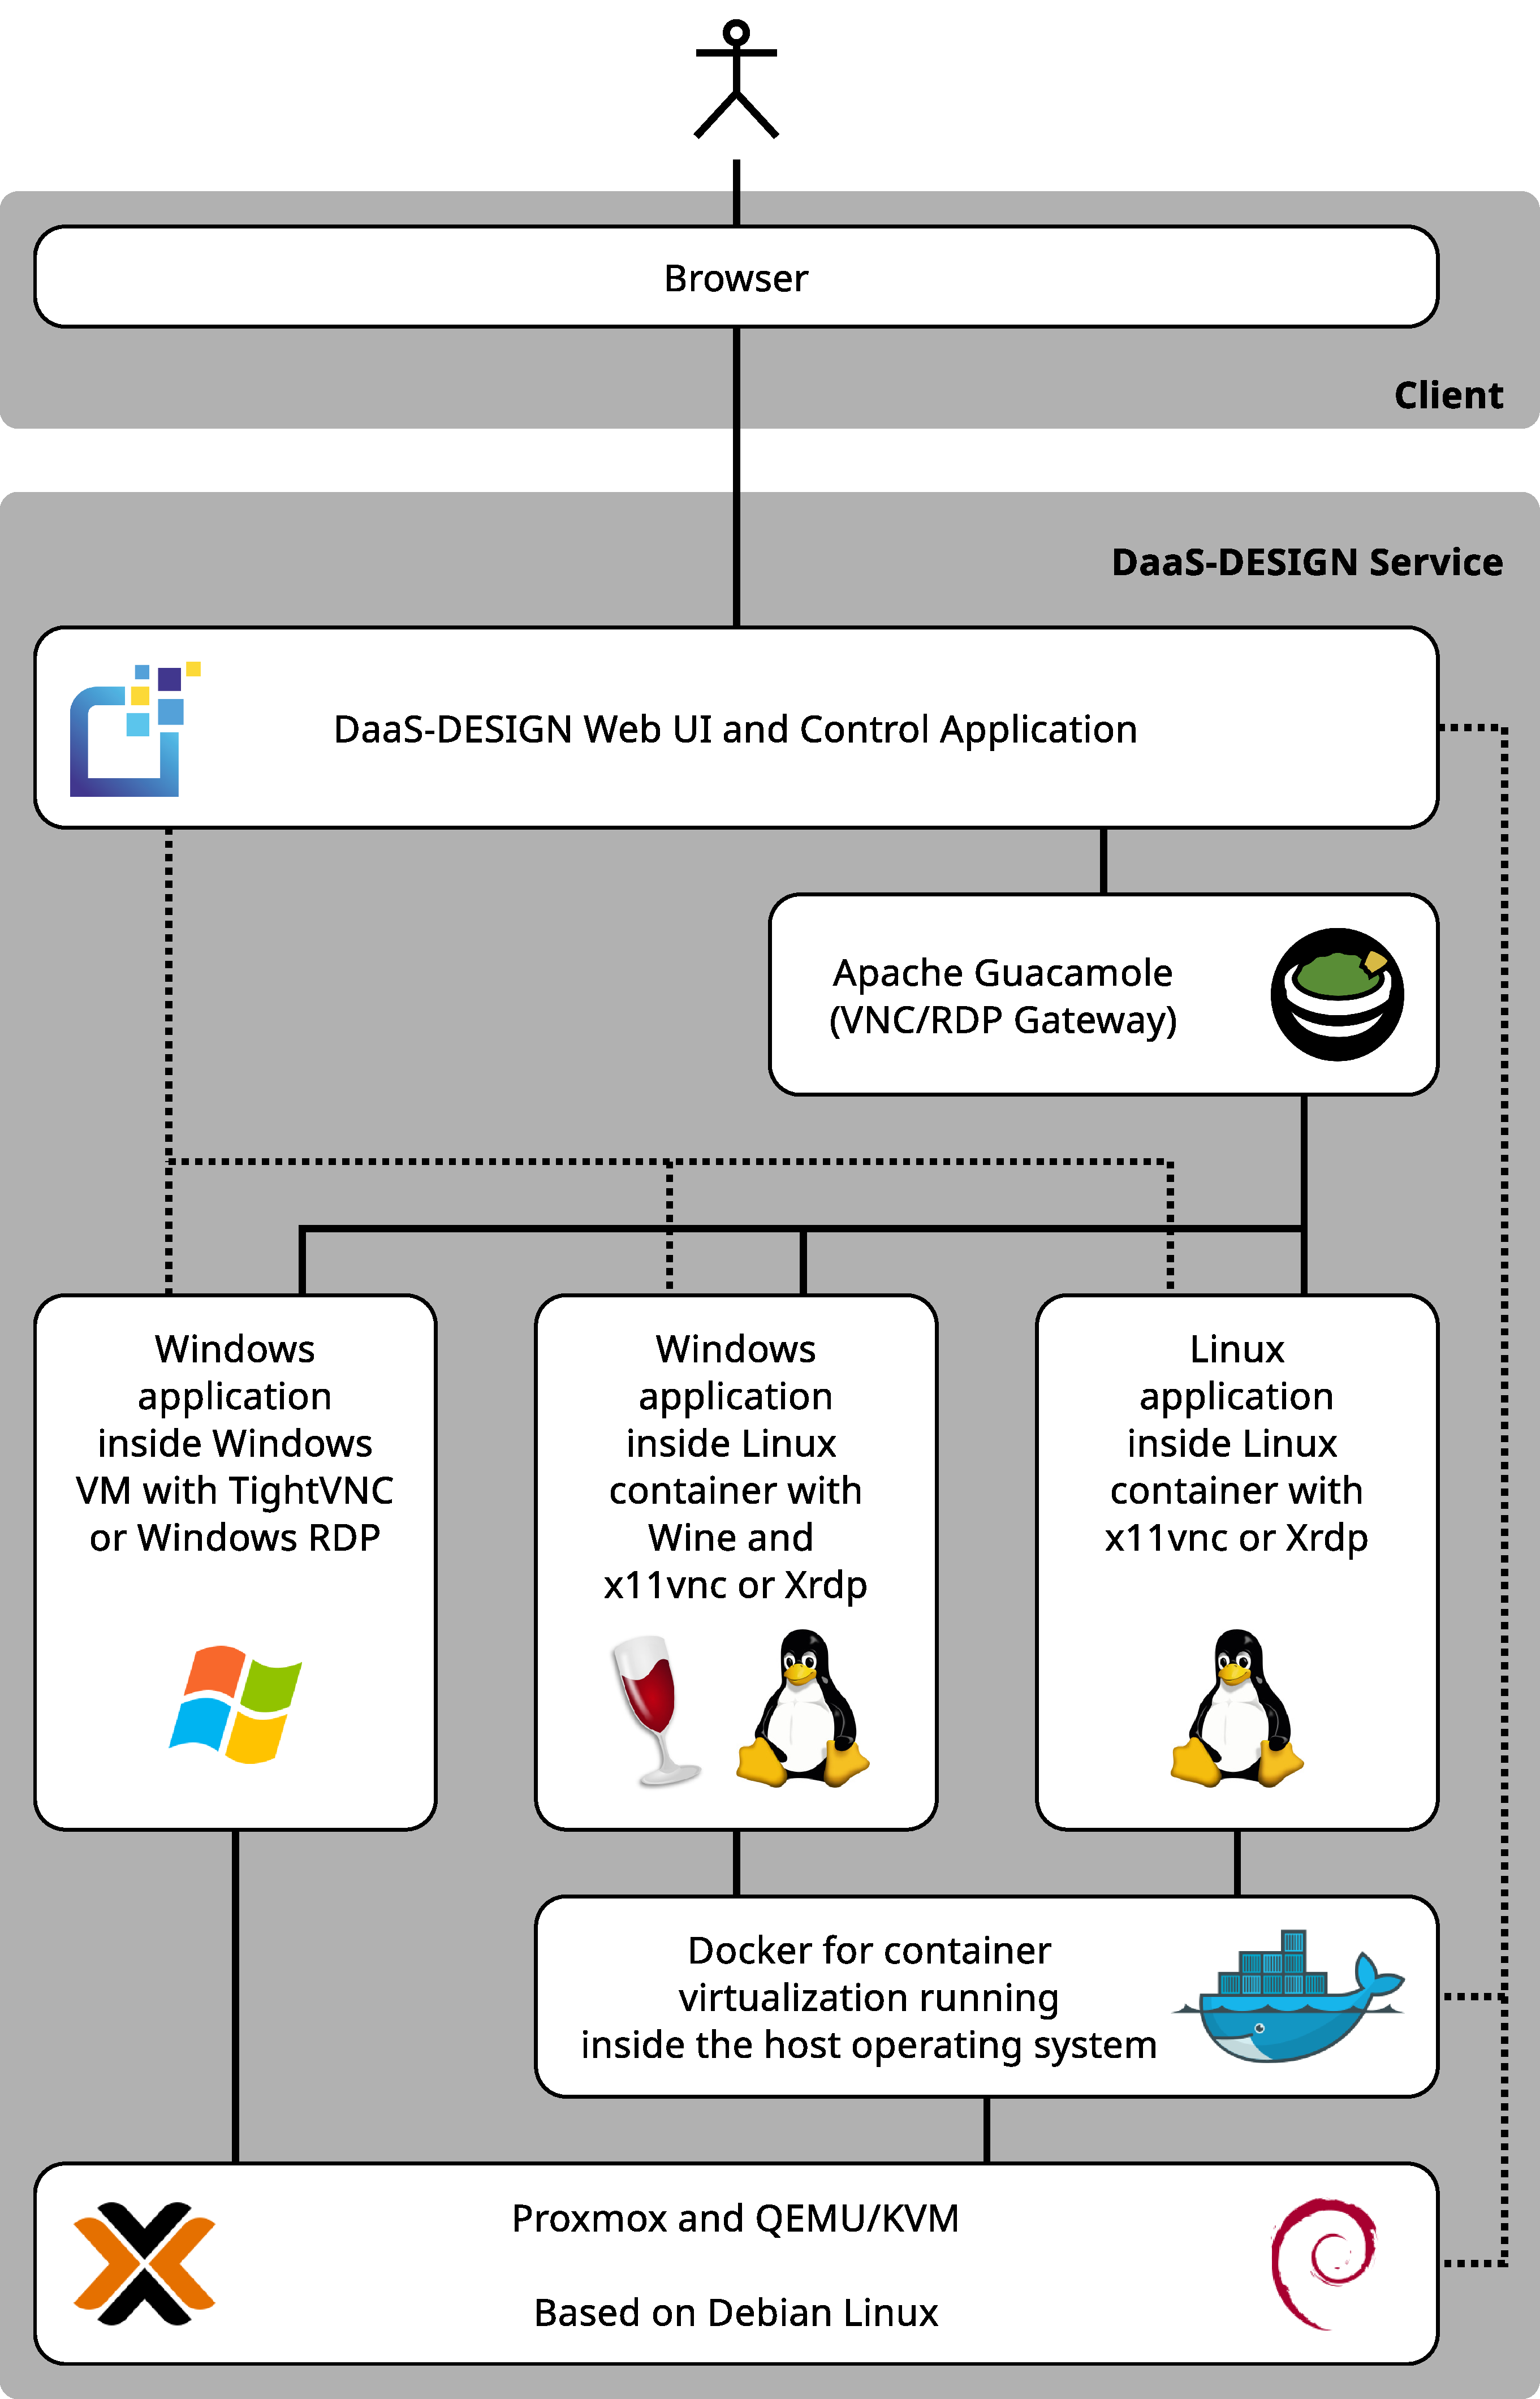
\includegraphics[width=\textwidth]{images/DaaS_DESIGN_Architecture_v11_english.pdf}
\caption{Architecture of the novel DaaS DESIGN.} \label{figure_architecture}
\end{figure}

\section{Challenges and Solutions}
\label{sec:AnalysisPossibleComponents}

TODO: Christian (1)
TODO: Johannes (2)

\subsection{Compatibility}

TODO: Christian (1)
TODO: Johannes (2)

Anwendungen (Windows / Linux / MacOS)

Sound (via sound-deamon oder via Guacamole)

Drucker (via cups oder via Guacamole)

Externe Geräte (USB-Stick)


\subsection{Performance}
% Initial brainstorm:
% + Welche Performance-Paramter / Kriterien sind hier relevant für die Anwendung / Nutzung
% + Fokus: Bottlenecks, Möglichkeiten der Performance-Steigerung, Grenzen/Limits, die man akzeptieren muss
% + Latenz hängt auch immer von Entfernung und Übertragungsmedium ab.
% + Skalierbarkeit: Stand und Möglichkeite
% + Ceph-Dateisystem
% + Datenbank SQlite aktuell. Perspektivisch MariaDB
% + Guacamole läuft 1x direkt auf dem Host aktuell. Läuft theoretisch auf jedem Host.
%
% Structure:
% performance of:
% - our serice itself
% - backend services
% - Viewer performance
% Limiting Factors
% - Hosting
% - Network
% - Internal data and communication
% Chosen techniques/solutions/protocols:
% - Filesystem (Ceph)
% - Database (sqlite, mariadb)
% - Guacamole (Proxy approach)
% Similar_Examples:
% - Cloud Gaming efforts 
%    - technical solutions, 
%    - latencies, 
%    - hardware support and integration)
%
% TODO: Johannes (1)
% TODO: Christian (2)
% TODO: Christian: Latenz bei Cloud-Gaming Erfahrungen
% TODO: 
%       - Include overall takeaway messages somewhere before:
%           - IaaS, PaaS and SaaS combined is defined as DaaS
%           - Define terms: Backend-service, Host-System, Instance
%           - We want a stable and usable system first, performance comes second
%           - Low effort to use and integrate is the most crucial aspect!!!
%           - No "Gamestation", but all modern applications shall be suported
%               - "Regular" office apps (Spreadsheets, Editor, Email, Filemanager)
%               - 3D modelling (Blender, Mayo, etc.)
%               - Audio/Video Editing? (kdenlive, Adobe Premiere, OBS?)
%               - Services (Webserver, Emailserver, Fileserver, etc.)
%           - If several solutions are plausible, implement all and let the user decide
%           - Give definitions for all specified daas-usecase
%       - More references
%       - Illustrate each subsection
%       - Typos, grammar, etc.

In order to describe the mission-critical performance aspects of our system,
we initially give a short overview on potential challenges,
inherent bottlenecks as well as other problem areas.
We do that with respect to the underlying usecase model of DaaS-Systems
and then follow with a more thorough description
of our own specific design decissions and particular solutions.

From our perspective, performance in general can be seen as the most crucial system property
which influences a majority of all other other relevant properties,
such as user experience, system responsivness and overall efficiency.
As a result, we had to address multifaceted
and potentially cross-concerning challenges
on several distinct layers within our own architecture.

From the core infratructure to backend services
and user-facing elements, each component inidvidually
has to achieve certain minimum requirements in its own domain
and in order to contribute to the overall performance goals of the whole system.
Hence, we outline key limiting factors that impede performance,
along with our experiences and tailored solutions
aimed at mitigating these challenges.
From our point of view the three most critial performance aspects
for Daas-Systems are:
\begin{itemize}
	\item Infrastructure and Platform
	\item Network Latency
	\item Internal Processing and Communication
\end{itemize}
As there is no generalized measurment system available,
we ordered them by their magnitude of impact
and based them to the best of our knowledge
on the obtained experiences during our research project.
Since each of them have their own characteristics,
specific behavior and requirements, implying a potential impact
on the overall system performance and resource utilization,
we describe them individually and in more detail
in the following seperate subsections.

\subsubsection{Infrastructure and Platform}
In general can be said, that the chosen infrastructure, platform and utilized software
may have the most influental impact on cpu and resource consumption
which has a dramatic impact on the overall system performance.
As a DaaS combines all aspects of IaaS, PaaS, SaaS into one system
each related performance characteristic has to be taken into account.

For Infrastructure-as-a-Service can be said
that our solution generally offers possibilities
to use either virtual machines or docker containers.
As can be seen in several scientific publications
discussing relevant performance aspects of such systems,
the obvious advanatge in most categories
has a lightweight container solution compared to virtual machine
if a identical program was tested in both environments
~\cite{felter2015updated}
~\cite{potdar2020performance}
~\cite{seo2014performance}.

On one hand, that implies for our solution,
that a container-based approach is most likely preferable,
if that choice is available.
On the other hand, that  choice is not always available,
as not every app can be run in a container-based environment.
In order to maximize coverage of possible apps being able to run on our system,
we offer container-based and virtual machine based application hosting
as a key concept of our solution.

As a second observation in the area of PaaS can be added
that in most studies there is no dramatic difference
if derivates of operating systems are compared to each other.
Nevertheless, there are derivates
which are more driven towards being lightweight and more performant
~\cite{boras2020performance}  %nix vs. nix win vs. win
~\cite{balen2020performance}. %win in vm
In cases where a Windows virtual machine can be replaced with a natively operating wine platform,
additional performance potentials can be leveraged
~\cite{huang2012performance}.  % win inside vm
In contrast to that if operating system of different types are compared to each other,
there are more obvious results
especially when taking into account implementations of low-level operating system functionality,
such as interrupt handling, memory allocation, driver-specific implementations
or other more subtle requirements such as boot time
or the time needed for maintenance or system updates
~\cite{sergeev2022docker} % docker, win vs nix
~\cite{sulaiman2021comparison}. % office apps win vs nix

As a result of our research we aim to spport
any Windows or Linux based operating system in virtual machines
but can only support Linux and Wine in containers
due to the fact that only terminal based Windows containers are supported by Microsoft.

\subsubsection{Network Latency and Bandwidth}
Another important aspect when providing web-based access to DaaS apps
is that also network latency and bandwidth play a very important role
which contribute to a large degree to the responsivenes of the system
directly experienced by the user.
As the user utilizes its application through a web browser
we aim to support standardized frame-buffer protocols
to enable user interaction and access to external devices such as printers or usb sticks.

Within such protocols and in cases where video content is transmitted,
the provided network bandwidth might be the main bottleneck
especially when it comes to high-resolution video streams.
In cases where audio, mouse movement or keyboard strokes are transmitted,
the network latency plays a more important role.
Therefore, the experienced responsivness and usability
crucially depends on the hosted application.

In general, such application specific requirements can to a certain degree be controlled
by protocol-inherent tuning parameters and utilized compression algorithms.
Therefore, our solution aims to maximize coverage of potential usecases
by offering several solutions and a set of appropriate tuning options
which intentionally forces the user to decide
which solution actually fits best for him.

For that purpose we utilize the desktop gateway implementation Guacamole,
which offers support for most utilized frame-buffer protocols VNC and RDP
as well as all relevant tuning options.
Guacamole not only implements out-of-the-box support for the protocols itself
but also adds the ability to integrate audio support for VNC or other external devices
as well as a javascript based webclient.

Nevertheless, in order to integrate guacamole into the system,
there are still things to consider which are not handled by guacamole
but would be assumed from a full fledged daas solution.

First and foremost must be considered how authentication is handled.
On one hand, from a daas system a user would expect the system to work
without forcing him to authenticate himself
to more than one authentication system and also only once per session.
On the other hand crucial information such as user passwords
might in general better be kept secret to the system,
such that users can not manipulate the provided system in an unintended way.
A potential problem arises if taken into account
that by default RDP requires a valid user session to the system.

For that particular reason guacamole was integrated
in a proxied approach by using proxied websockets.
This enables to keep credentials of the generated system secret to the host system
while still providing authorized but passwordless access to the hosted application.

Further the proxy mechanism enables to support dynamic desktop resizing
which is a default guacamole feature for RDP,
but which is not available in VNC through guacamole.
By intercepting websocket opcodes and listening for size requests,
the requested resolution can then be enforced
by directly interacting with the related container or virtual machine.

Both changes to the default guacamole usecase are mandatory
in order to comply with the requirements for the underlying daas design
but both also impact the overall system performance and responsiveness in a negative way.
From a network perspective the integration as proxy adds an additonal network hop
and leads to a noticable delay in the network communication.
The protocol level evaluation of opcodes enhances that delay additonally
and the perceived responsiveness might suffer
if resize requests take more time then expected.
Overall, the introduced overhead is still acceptable
and enables platform-independent and seamless access for all defined daas usecases.

\subsubsection{Internal processing and Communication}
Another important aspect directly related with performance and responsiveness
is the approach in which data is internally processed, stored and communicated
to all involved components and instances.
This includes the metadata being collected and processed by essential components
but also implies raw physical data being directly exchanged with object instances.

In order to provide a satisfying user experience in a daas system
certain components in a host system are required.
This includes access to all backend services
being used to create containers and virtual machines,
a local or remote database, a local or remote authentication service,
local and distributed filesystems as well as
virtual or physical network devices.
Further a webserver is integrated to provide all relevant api endpoints
for the frontend communication
as well as all websocket endpoints for the viewer communication.

Generally spoken all of these components might become a potential bottleneck
when being utilized with high throughputs
or large amounts of concurrent applications demanding low latencies.
This is especially the case if being used in a sequential manner
or being served from the same hardware.
The total time needed for a request being fully processed
can increase drastically if delays add up to each other.

On a architectural level all relevant components are therefore designed
for being distributed to different hosting systems
if requirements of a certain user scenario suggests it.
Nevertheless, it might still be advisable
to keep certain components directly on the host system
in order to ensure low latency component access.

For all components with realtime and low latency usecases it is generally advisable
to keep them as close to the core hosting system as possble.
This includes all data and communication
relevant to audio, video, mouse and keyboard transmission,
but also the relevant backend-service to host containers and virtual machines.
That might be in the best case to host them natively on the host itself
which enables virtual network and hardware access.
In the worst case that might be at least connected to the same physical network
in order to reduce network latencies as much as possbile.

For all other components of overarching nature
such as database access, authentication provider and filesystems
it is still advisable to keep a close distance to the host
but it also highly depending on the total amounts of users
and the specifics of their usecases.
In small scales it is still advisable to keep such components on the same system
but in larger scales it preferable to externalize such functionality to dedicated systems.


\subsection{Stability}
% TODO: Johannes (1)
% TODO: Christian (2)
% TODO: Johannes: Beschreibung zur Position der Komponenten, Möglichkeiten der Parallelisierung und Einschränkungen
%
% Was ist hier relevant?
% Verfügbarkeit des Service und der Benutzerdaten
% Redundante Komponenten (Hardware und Software)
% Welche Komponenten kann man sinnvoll redundant vorhalten?
% Was sind die Vor- und Nachteile?
% Auch Kosten?
% Wo sehen wir aktuell in unserer Architektur Risiken für Dienstausfall und Datenverlust?
% Features von Proxmox
% Ceph-Dateisystem
% Datenbank SQlite aktuell. Perspektivisch MariaDB
% Guacamole läuft 1x direkt auf dem Host aktuell. Läuft theoretisch auf jedem Host. Proxmox kann sich darum kümmern?!
% Docker haben/nicht haben / Vor- und Nachteile
% Hier auch auf die Skalierbarkeit beziehen
% Structure:
%	- Stability
%		- Redundancy
%		- Scalability
%	- Backend-services
%		- Database
%		- Authentication
%		- Distributed Filesystem
%		- Container/VM (Proxmox, Kubernetes?) 
%		- Instance error => Recreate
%	- Considerations:
%		- Divide and conqueror
%		- Requirement: Distributable components
%	- Risks:
%		- Filesystem error
%		- Database error
%		- Authentication error
%		- Infrastructure error (Container/VM)
%	- Benefits/Drawbacks:
%		- Distribution of components is distribution of load => Performance
%		- Eliminates bottlenecks
%		- Errors affect only errornous component


Stability in Desktop as a Service (DaaS) applications is of major importance
to ensure that our solution can meet the demands of continuous
and time-critical operations across varied user scenarios.
From our point of view any daas system must ensure the stability
of all system components during runtime
in order to maintain the ability to provide service continuity,
handle growing user loads and to transparently recover from failures,
while still providing a seamless end-user experience.
Such considerations are an integral part of our architectural concept
as they directly impact the operational integrity
of the system and its hosted instances,
making them suitable for enterprise-level deployment and trust.

This definition of stability is underpinned by several architectural
and operational strategies including redundancy of components, scalability of nodes,
and a robust backend service framework
providing means of communication between components and nodes.
These strategies as well as their drawbacks and benefits
will be further discussed on a component level
and within the following subsections.

\subsubsection{Scalability of Components}
Scalability in general, but also specificaly in daas environments
can be approached in two fundamental ways:
horizontal and vertical scaling.
Horizontal scaling, or scaling out, involves adding more machines or instances
to a pool to manage increased load.
In contrast to that, vertical scaling or scaling up,
refers to adding more power (CPU, RAM)
to an existing machine~\cite{vaquero2011dynamically}.

While horizontal scaling is generally more flexible
and often preferred in cloud environments
due to its ease of integration with existing architectures,
vertical scaling remains important for applications
requiring strong single-thread performance or low latencies.

In order to comply to both we defined means of configuration
such that the system itself as well as all of its backend services
are designed to be split up into logical units
which can be distributed to dedicated systems.
Esssentially, all backend services receive their own dedicated configuration
and can be accessed via tuples of hostname and port.
Any component using such a backend service can obtain the relevant tuple
and then use it to fetch requests from that service.
By default and in a standlone configuration
all backend-services reside on the same native host
and relevant tuples can be derived from the host configuration.
In a distributed context a selection of these services
can be distributed to a dedicated and remote system
in order to comply to horizontal scaling principles.
The relevant tuple can then be derived from any node in the system
by utilizing a common database containing the relevant metainformation.

Vertical Scaling of daas nodes is currently not planned
but a adminstrators are free to use custom 3rd party toolchains, e.g for GPU virtualization.
Allthough vertical scaling on a host basis
is beyond scope of our research project,
it is more plausbile to scale the instances
being hosted within that system and for both dimensions.

For vertical scaling of instances appropriate parameters and api endpoints are present
in order to manipulate the configuration of their resource assignments,
such that arbitrary configurations are possible.

For horizontal scaling of instances
the builtin mechanisms of each backend service are automatically configured and utilized
such that instances can be arbitrily distributed across a pool of connected nodes.
In the case of virtual machines the responsible backend service proxmox implements
such mechanisms as part of its 'Proxmox VE High Availability (HA)' cluster.
In the case of containers any backend service fullfilling
similar concepts can be integrated, as for example with kubernetes.
Within such clusters any daas instance is fully agnostic to its hosting system
and must only be reachable via a known hostname or ip.

\subsubsection{Redundancy of Components}

Redundancy is critical for most distributed systems
but especially for daas architectures,
and serves as a safeguard against service interruptions and data loss
by duplicating essential components, functions and data.
This design principle ensures that systems remain highly available and reliable,
even during component failures.
In the following a list of components eligable for redundancy is given
which briefly describes the most relevant strategies contained in our architecture.

\begin{itemize}
	\item \textbf{Frontend/Backend: } In our final version
	      redundancy of the frontend and backend components will offer means of configuration
	      such that multiple instances can be distributed to dedicated systems
	      and can be target of standardized load balancing strategies.
	      By doing so the frontend or the backend may just act as a gateway
	      between the user and the backend service containing the relevant instances.
	      In that manner redundancy is achieved and frontend or backend
	      can forward requests and responses
	      by identifying the correct communication endpoint
	      based on url's or specific parts of them,
	      as for example by extracting hostnames
	      or specific identifiers being unique within the daas domain.
	\item \textbf{Database: } The database is integrated as a backend service
	      and as such completely unaware of surrounding components
	      and contexts in which it is used.
	      The database can therefore be distributed to a dedicated system if needed.
	      Generally, any modern database (e.g. MariaDB) implements rich features
	      to maintain specific data consistency strategies
	      such as data replication, clustering,
	      dedicated failover mechnisms or also RAID control.
	      Therefore redundancies of our database system are currently not planned,
	      but can easily be applied by users with such needs
	      and by using database specific features and a modified database adapter.
	\item \textbf{Authentication: } Authentication within our architecture
	      is also implemented as a backend service
	      and can therefore be distributed to any dedicated system,
	      can be a target of standardized load balancing mechanisms and strategies
	      and is as well fully agnostic of surrounding components
	      and calling contexts.
	      The authentication system maintains
	      its own credential registry in a seperate database,
	      a customizable set of user and group privileges,
	      and implements the well defined OAuth 2.0 standard
	      to allow remote authentication.
	      In our final version, a customizable amount of redundant systems might be configured.
	      % TODO: Discuss: Is that true? Do we want to make Darios authenticator redundant?
	\item \textbf{Distributed Filesystem: } Within our architecture
	      we use the distributed filesystem ceph which is a distributed storage system
	      providing object, block and file storage. In ceph redundancy is achieved
	      through its self-healing and self-managing capabilities utilizing an algorithm
	      called CRUSH (Controlled Replication Under Scalable Hashing).
	      Data availability and fault-tolerance is obtained
	      by automatically managing replication
	      of data pieces across different devices.
	      Our designed architecture uses these capabilities
	      to reliably provide
	      file storage to host systems and all hosted daas instances
	      and provides block storage to the infrastructural backend services.
	      By hosting daas instances directly from the distributed block storage,
	      arbitrary redundancy scenarios might be covered
	      by using specific configuration parameters.
	\item \textbf{Instances: } Redundancy of instances
	      is not a necessary condition for daas systems in general
	      but it might make sense to apply such strategies under certain conditions.
	      By using highly available clusters within our backend services
	      redundancy can simply be achieved by using the corresponding api endpoints
	      previously described and by parameterizing them appropriately.
\end{itemize}

\subsubsection{Internal Communication}
After discussing the principles being used to achieve scalability and redundancy
it adheres to describe how communication flows are maintained
in such a distributed enironment.

Our proposed solution is at the core designed
as a message oriented architecture
which additionally aims to fullfill daas properties
for scalability and redundancy as previously described.

That implies fundamentally, that any action being triggered,
may it either be in the frontend on the client side,
in the backend on the host side
or within any of the hosted instances
must always fullfill the condition that the required information to execute that action
must either be directly derivable from a request or a corresponding response
or otherwise, must be immidiately available to the component executing that action.

We achieve that by storing all runtime information of instances in the distributed block storage,
by storing all relevant configuration files in our distributed file storage,
by utilizing a common database to persist all object metadata
and by using our decentralized OAuth component to handle authentication.

By doing so, any change being trigerred by a node within the daas network
is immidiately available to any other node in the system
which relies on that information change.
Apart from that any additional information needed by a component
is fully contained within the related request or response.

Therefore, arbitrary distributed configurations are possible
as long as request and response messages reach their desired target eventually
and as long availability of all relevant backend services is guaranteed.

If that is the case, each distributed daas node can typically
just contain all time-critical components as a bare minimum
in order to maintain an acceptable performance throughout the whole user-facing network stack.
This would typically include the backend service hosting the relevant instances
as well as the websocket proxy directly connected to the guacamole daemon
and all other components may reside somewhere in the daas network.


\subsection{Usability}

TODO: Christian (1)
TODO: Johannes (2)

Ideen und Konzepte zur Trennung von User und Admin-Ansicht

Reduktion der Komplexität der Bedienung durch Fokus auf notwendigste Interaktionsschritte

Desktop vs. einzelne Anwendung im Browser-Tab

Anpassung des Browser-Inhalts auf die Größe der Anwendung

Herausforderungen, Entwicklung, Implementierung, Lessons-learned

TODO Johannes: Erlebnisse der letzten 3-4 Wochen aufschreiben



\section{Conclusion}
\label{sec:Conclusions}

TODO: Zusammen am Schluss

\section{Outlook}
\label{sec:NextSteps}

TODO: Zusammen am Schluss

\section*{Acknowledgements}

This work was funded by the Federal Ministry for Economic Affairs and Climate Action
('\textsl{Bundesministerium f\"ur Wirtschaft und Klimaschutz}')
in the framework of the central innovation programme
for small and medium-sized enterprises
('\textsl{Zentrales Innovationsprogramm Mittelstand}').

We thank our project partners from Nuromedia GmbH for their support.
We especially thank Björn Goetschke, Mike Ludemann, Dario Savella, Holger Sprengel, and Rahul Tomar.



% ---- Bibliography ----
%
% BibTeX users should specify bibliography style 'splncs04'.
% References will then be sorted and formatted in the correct style.
%
\bibliographystyle{splncs04}
\bibliography{biblio}
%

% \bibliography{\jobname_no_dashes_at_repeated_names,references}{}


\end{document}
